\section{\Cyclus Simulator Paradigm }

The \Cyclus project at the \gls{UW} at Madison is the 
simulation framework in which this repository model is designed to 
operate.  Modular features within this software architecture provide a 
great deal of flexibility, both in terms of modifying the underlying 
modeling algorithms and exchanging components of a fuel cycle system.

The \Cyclus fuel cycle simulator is the  result of lessons learned 
from experience with previous nuclear fuel cycle simulation platforms.  
The modeling paradigm follows the transaction of discrete quanta of 
material among discrete facilities, arranged in a geographic and 
institutional framework, and trading in
flexible markets. Key concepts in the design of \Cyclus include open
access to the simulation engine, modularity with regard to
functionality, and relevance to both scientific and policy
analyses. The combination of modular encapsulation within the
software architecture and dynamic module loading allows for robust but 
flexible reconfiguration of the basic building blocks of a simulation 
without alteration of the simulation framework.  

The modeling paradigm adopted by \Cyclus includes a number of
fundamental concepts that comprise the foundation on which other, more
flexible, design choices have been made. 

%%%%%%%%%%%%%%%%%%%%%%%%%%%%%%%%%%%%%%%%%%%%%%%%%%%%%%%%%%%%%%%%%%%%%%%%%%%%%%%%
\subsection{Dynamic Module Loading}

The ability to dynamically load independently constructed modules is a
heavy focus of \Cyclus development. Dynamically-loadable modules are
the primary mechanism for extending \Cyclus' capability. The primary
benefit of this approach is encapsulation: the trunk of the code is
completely independent of the individual models. Thus, any
customization or extension is implemented only in the loadable
module. A secondary benefit of this encapsulation is the ability for
contributors to choose different distribution and licensing strategies
for their contributions. By allowing models to have varied
availability, the security concerns of developers can be
assuaged (See Figure \ref{fig:repo}). 

\begin{figure}[htb!]
  \begin{center}
    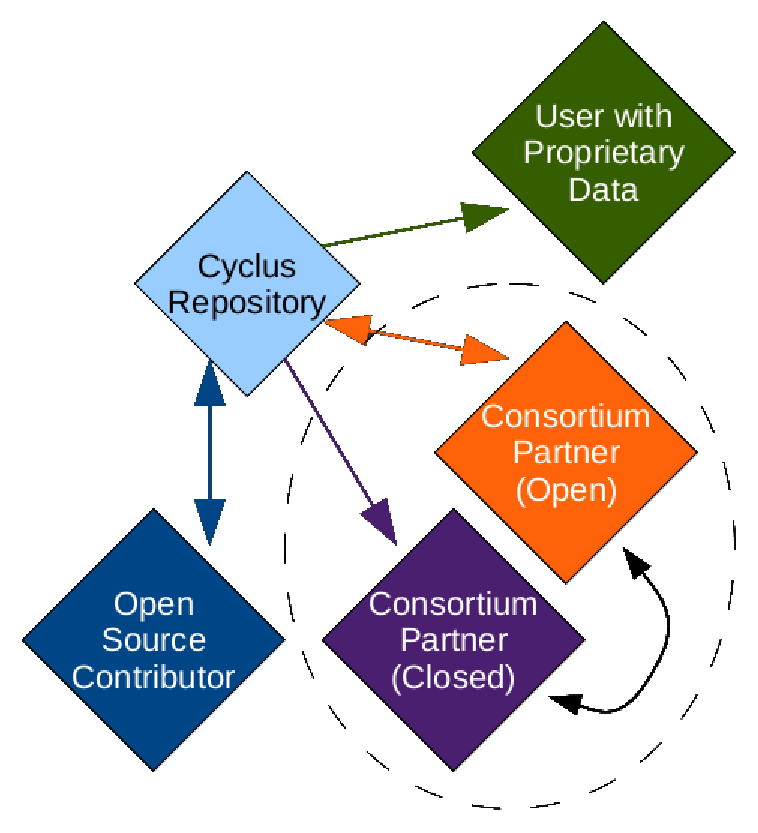
\includegraphics[width=0.5\textwidth]{./chapters/paradigm/openness.eps}
  \end{center}
  \caption{The \Cyclus code repository allows for varied accessibility.}
  \label{fig:repo}
\end{figure}

Finally, this strategy allows individual developers to
explore different levels of complexity within their modules, including
wrapping other simulation tools as loadable modules within the \Cyclus 
framework. This last benefit of dynamically-loadable modules addresses 
another goal of \Cyclus: ubiquity amongst its potential user base. By
engineering \Cyclus to easily handle varying levels of complexity, a single
simulation engine can be used by both users interested in big-picture policy
questions as well as users focused on more detailed, technical
analyses.

%%%%%%%%%%%%%%%%%%%%%%%%%%%%%%%%%%%%%%%%%%%%%%%%%%%%%%%%%%%%%%%%%%%%%%%%%%%%%%%%
\subsubsection{Encapsulation}

\Cyclus implements an encapsulated structure that takes advantage of 
object-oriented software design techniques in order to create an 
extensible and modular user and developer interface. A primary 
workhorse for this implementation is the notion of dynamic module 
loading in combination with  well defined module interfaces within 
a region, institution, and facility  hierarchy. In this paradigm, 
the shared interface of polymorphic objects is abstracted from the 
logic of their instantiation by the model definition they inherit.  

In this way, \Cyclus allows a level of abstraction to exist between 
the simulation and model instantiation as well as between model 
instantiation and behavior.  An interface defines the set of shared 
functions of a set of subclasses in an abstract superclass. In \Cyclus
main superclasses are Regions, Institutions, and Facilities 
while their subclasses are the concrete available model types (e.g. a 
RecipeReactorFacility). See Figure \ref{fig:modularity}.

The interface for the FacilityModel class is the set of 
virtual functions declared in the Facility class such as getName, 
getID, executeOrder(), sendMaterial(), receiveMaterial() etc.  Through 
such an interface, the members of a subclass can be treated as 
interchangeable (polymorphic) instantiations of their shared 
superclass. 

\begin{figure}[htb!]
  \begin{center}
    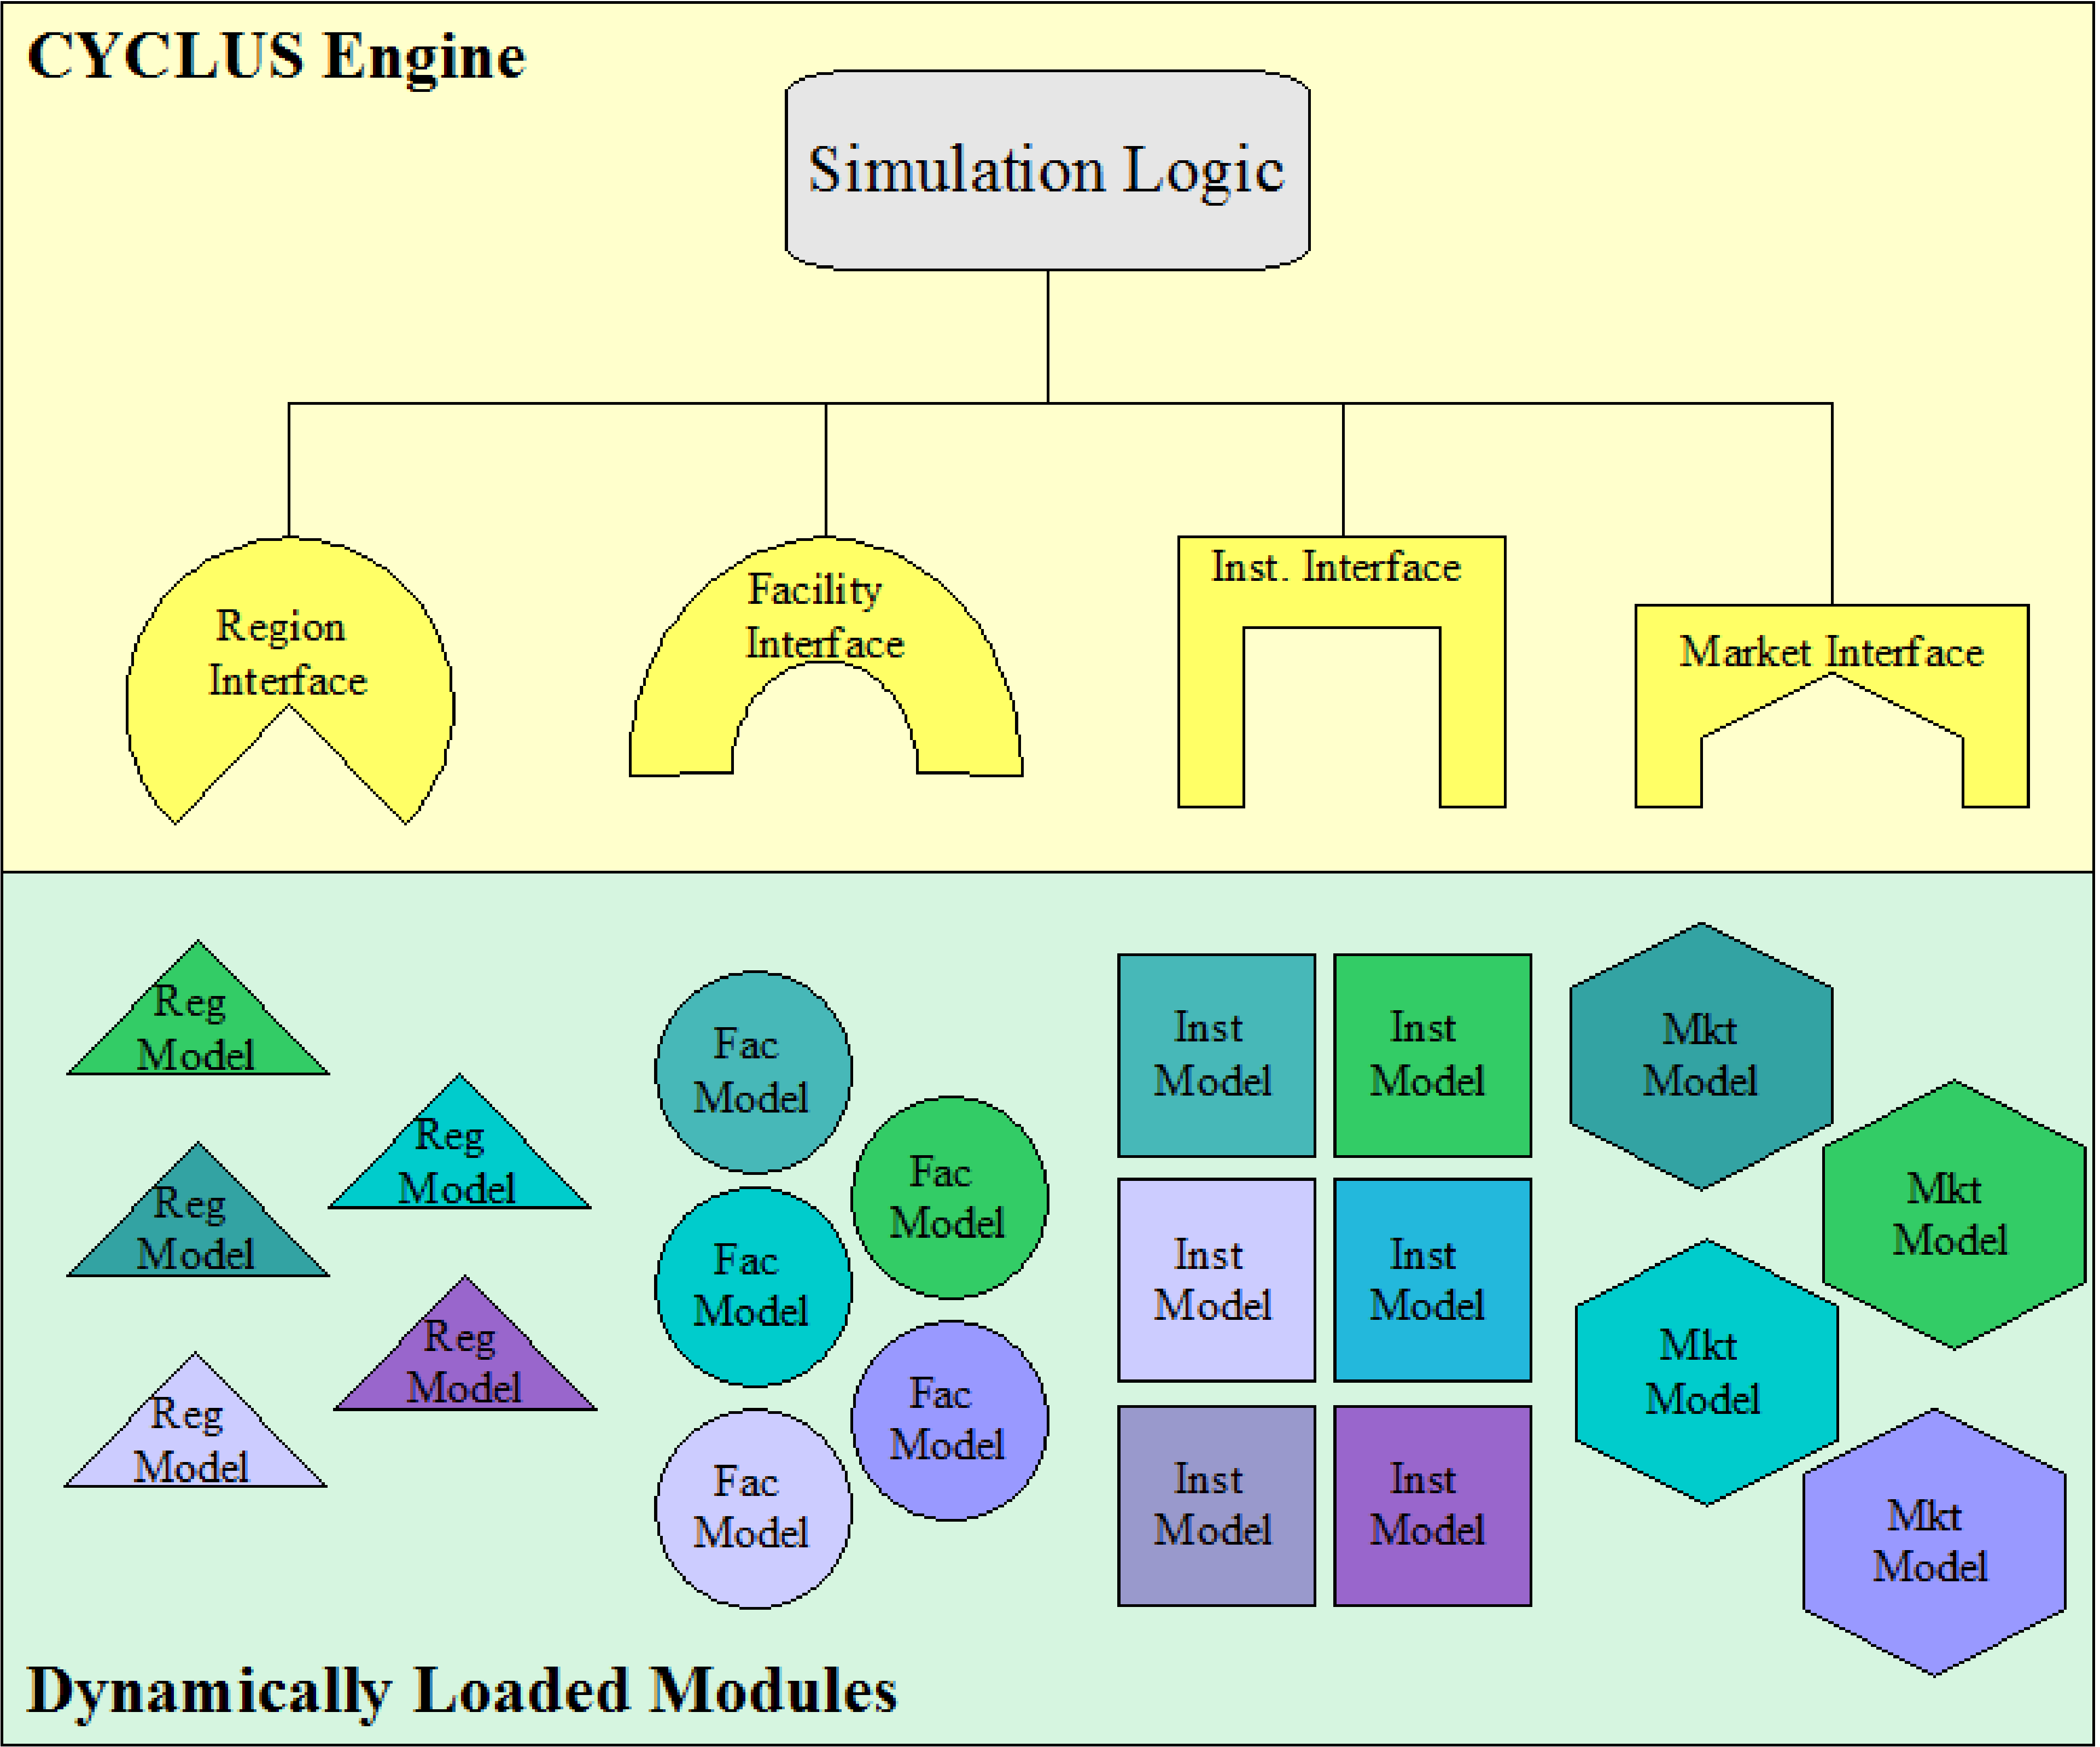
\includegraphics[width=0.7\textwidth]{./chapters/paradigm/modularity.png}
  \end{center}
  \caption[Module Interfaces and Encapsulation]{Modules are defined solely 
  by their interfaces in a modular paradigm and can be arbitrarily 
  interchanged with modules posessing equivalent interfaces.}
  \label{fig:modularity}
\end{figure}


%%%%%%%%%%%%%%%%%%%%%%%%%%%%%%%%%%%%%%%%%%%%%%%%%%%%%%%%%%%%%%%%%%%%%%%%%%%%%%%%
\subsubsection{Modularity and Extensibility}

A modular code must have the traits of encapsulation and abstraction 
appropriate for a user or developer to flexibly make alterations to 
the simulation performance with minimal modification to the code. An 
extensible code should be both robustly suited to the addition of 
classes and subclasses as well as suited to communication with other codes.
In \Cyclus, addition of new models by dynamic loading is possible without 
any alteration of the software trunk. The modular design of \Cyclus stresses
avoidance of rigidity, in which changes to the code are potentially difficult, 
and fragility, in which changes to the code are potentially damaging.

%%%%%%%%%%%%%%%%%%%%%%%%%%%%%%%%%%%%%%%%%%%%%%%%%%%%%%%%%%%%%%%%%%%%%%%%%%%%%%%%
\subsection{Market-based Material Transactions}

The foundation of a simulation is a commodity market that collects 
offers and requests and matches them according to some algorithm.  The 
user is able to select which type of algorithm is used for each market 
by selecting a MarketModel and configure it with a particular set of 
parameters defined by that MarketModel.  Changing the parameters of a 
market changes its performance and selecting a different MarketModel 
completely changes its behavior.

The transaction of nuclear materials takes place in markets that act
as brokers matching a set of requests for material with a set of
offers for that material. A variety of market models will be available
to perform this brokerage role. It is important to note that each
market is defined for a single commodity and acts independently of
other markets. Once the requests and offers have been matched by each
market in a simulation, the facilities exchange material objects.

Facilities are deployed to issue offers and requests in these markets.  
Like markets, the user may select which type of algorithm is used for 
each facility by selecting a FacilityModel and configure it with a 
particular set of parameters defined by that FacilityModel.  Changing 
the parameters of a facility changes its performance and selecting a 
different FacilityModel completely changes its behavior.  Unlike 
markets, multiple independent instances of each facility configuration 
can be deployed to represent individual facilities.


%%%%%%%%%%%%%%%%%%%%%%%%%%%%%%%%%%%%%%%%%%%%%%%%%%%%%%%%%%%%%%%%%%%%%%%%%%%%%%%%
\subsection{Discrete Materials and Facilities}

The \Cyclus modeling infrastructure is designed such that every
facility in a global nuclear fuel cycle is treated and acts
individually. While modeling options exist to allow collective
action, this will be as a special case of the individual facility
basis. Each facility has two fundamental tasks: the transaction of
goods or products with other facilities and the transformation of
those goods or products from an input form to an output form.  For
example, a reactor will receive fresh fuel assemblies from a fuel
fabrication facility, transform them to used fuel assemblies
using some approximation of the reactor physics, and supply those used
fuel assemblies to a storage facility.

A facility configuration is created by selecting a FacilityModel and 
defining the parameters for that facility configuration.
Each FacilityModel will define its own set of parameters that 
govern its performance.  The same FacilityModel may be used for 
multiple facility configurations in the same region, each with 
parameter values appropriate for that facility configuration.

The repository model that is the subject of this work is a facility 
model within the \Cyclus simulation paradigm. 

%%%%%%%%%%%%%%%%%%%%%%%%%%%%%%%%%%%%%%%%%%%%%%%%%%%%%%%%%%%%%%%%%%%%%%%%%%%%%%%%
\subsection{Materials}

Material movement is the primary unit of information in \Cyclus.  
Materials passed, traded, and modified between and within facilities 
in the simulation are recorded at every timestep.  This material 
history is stored in the output dataset of \Cyclus. In addition to 
holding the map of isotopes and their masses, a material object holds 
a comprehensive history of its own path as it moves through models 
within the simulation. 

\subsection{Implications for Repository Model}

The above sections outline the fuel cycle simulation platform
currently under development at \gls{UW} in which the repository model
at hand is to be implemented.  Implemented as a facility within this 
framework, the repository model interface is defined by the Facility
Model interface defined within the \Cyclus paradigm. 

That interface requires that a capacity be defined by the repository at every 
\Cyclus timestep so that the repository may make appropriate requests of 
disposable material.

Furthermore, the capability for dynamic module loading possible within 
the \Cyclus paradigm allows the repository system subcomponents to be 
interchangeably loaded at runtime, enabling comparison of various 
repository subcomponents, physical models of varying levels of detail. 

The repository is both a subclass and a superclass. It is a subclass of the 
FacilityModel class, and a superclass of its own subcomponents. That is, 
dynamically loaded subcomponents of the repository inherit data, parameters and 
behaviors from the repository itself. 


%%%%%%% As Paul Dirac once said. . . In science one tries to tell
%%%%%%% people, in such a way as to be understood by everyone,
%%%%%%% something that no one ever knew before. But in the case of
%%%%%%% poetry, it's the exact opposite!


